\documentclass{ctexart}
\usepackage{amsmath}
\usepackage{geometry}
\usepackage{hyperref}
\usepackage{graphicx}
\usepackage{float}
\author{陈启钰\,\, 2300011447}
\title{三线摆实验}
\date{\today}
\begin{document}
	\maketitle
	\section{传统实验方法简述}
	\subsection{实验原理}
	如图\ref{fig:sxb}所示,其中悬盘$O_1A_1B_1C_1$ 被三根等长的细线分别过等距离的三点$A_1$、$B_1$和$C_1$水平地悬挂于固定盘$OABC$上等距的三点$A$、$B$和$C$。若悬盘的质心位于$O_1$点,可以证明,在保证$OO_1$轴竖直,且摆角振幅$\theta_0$很小的条件下,悬盘会绕$OO_1$轴作近简谐的扭摆运动,其扭摆周期$T$满足
	\begin{align}
		T^2=\frac{4\pi^2HI}{m_0gRr}
		\label{eq:T}
	\end{align}
	从而转动惯量
	\begin{align}
		I=\frac{mgRr}{4\pi^2H}T^2
	\end{align}
	\begin{figure}[H]
		\centering
		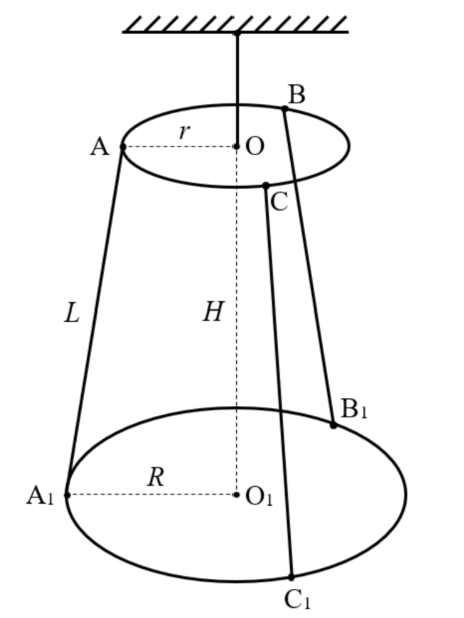
\includegraphics[width=5cm]{sxb.png}
		\caption{三线摆示意图}
		\label{fig:sxb}
	\end{figure}
	式中$H$是三线摆处于平衡位置时固定盘下表面到悬盘上表面的距离;$r$和$R$分别是$OABC$和$O_1A_1B_1C_1$的半径;$I$是悬盘对$OO_1$轴的转动惯量;$m_0$是悬盘的质量;$g$是重力加速度。这里,除质心位置外,对悬盘的质量分布并未作任何限制。如果将待测物体固定在悬盘上,使整体的质心位置仍在$OO_1$连线上,式\ref{eq:T}中的$I$就应该是悬盘与待测物体对$OO_1$轴的转动惯量之和。
	\subsection{实验过程}
	\paragraph{测量仪器常数}测定仪器常数$l$、$R$、$r$和$m_0$。
	\paragraph{悬盘的转动惯量}悬盘上不放置待测物体,使三线摆做扭转运动,测量得到周期$T_0$,利用已知的三线摆参数计算出悬盘本身的转动惯量$I_0$。
	\paragraph{测量物体的转动惯量}将待测物体固定到悬盘上,使整体做扭转运动,测量得到周期$T_1$,计算得到悬盘和待测物体的总转动惯量$I_1$(注意式中质量应该代入总质量)。待测物体的转动惯量为$I_1-I_0$。
	\section{线性回归方法}
	在没有放置任何工件的时候,对于三线摆系统,在加上质量$m_i$,转动惯量$I_i$的工件的时候,有
	\begin{align}
		T^2=\frac{4\pi^2H(I_0+I_i)}{(m_0+m_i+m)gRr}
	\end{align}
	式中$m$为配重的质量,需保证$m_0+m_i+m=M$是一个常数($m$可变),此时即有
	\begin{align}
		T^2=\frac{4\pi^2H}{MgRr}I_i+\frac{4\pi^2H}{MgRr}I_0
	\end{align}
	对$T^2-I_i$进行线性拟合,得到
	\begin{align}
		T^2=KI_i+B,K=\frac{4\pi^2H}{MgRr},B=\frac{4\pi^2H}{MgRr}I_0
	\end{align}
	从而$I_0$可以计算得到
	\begin{align}
		I_0=B/K
	\end{align}
	从而得到悬盘的转动惯量,同理也可以得到待测工件的转动惯量。
	\section{实验开始的调节的状态}
	\noindent 三线摆底座调至水平状态。\\
	调节悬盘、垫盘和底座平行。\\
	三根悬线长度相同且绳上张力相同。\\
	光电门位于挡光片平衡位置附近。
	\section{注意的要点}
	\noindent 三线摆底座、悬盘、垫盘保持水平。\\
	摆线长度不能过短否则不满足小角度近似。\\
	对于测量周期数的选取,要满足误差等量分配原则。\\
	系统的质心需要始终保持在悬点正下方。\\
	释放三线摆时可以通过扭转的方式以减小摆动对实验造成的影响。
	\section{相比传统方法的优点}
	\noindent 可以忽略小角度近似不满足、系统摆动、质量改变等条件对实验造成的影响。\\
	采用测量多组数据进行线性拟合的方式,与原来只测量两个周期相比可以减小实验测量误差。
\end{document}